%!TEX root=../document.tex

\section{Einführung}


\subsection{Ziele}

\subsection{Voraussetzungen}

%Listen erstellen
%\begin{itemize}
%	\item \textbf{ \"Ubungsteil 1:} 
%	\item \textbf{ \"Ubungsteil 2: } 
%\end{itemize}

%Bilder einfügen
%\begin{figure}[!h]
%	\begin{center}
%		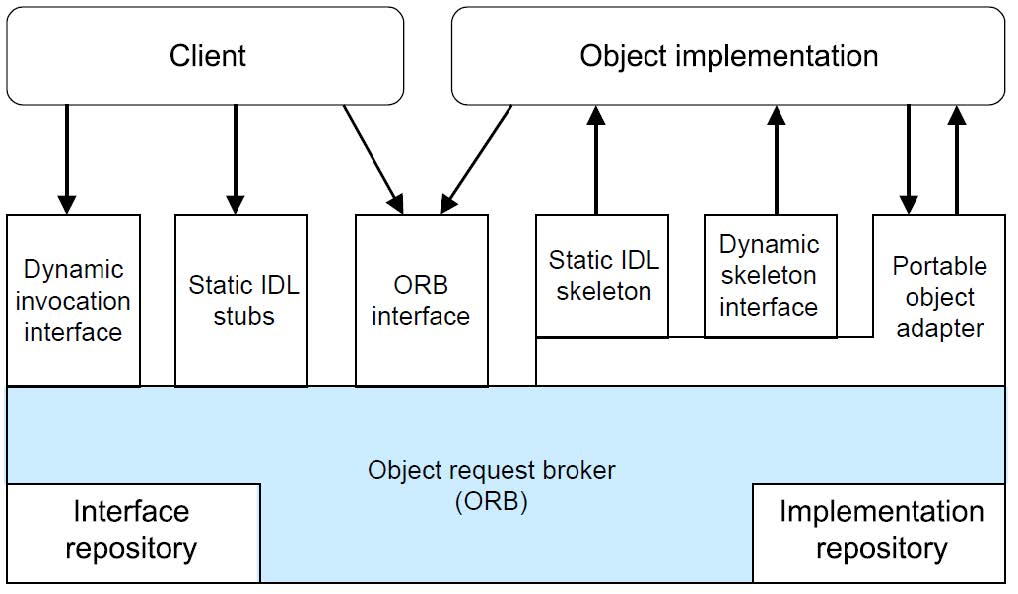
\includegraphics[width=0.5\linewidth]{images/corba.jpg}
%		\caption{Common Object-Request-Broker Architecture \cite{tanenbaum2007verteilte}}
%		\label{broker}
%	\end{center}
%\end{figure}
%

\subsection{Aufgabenstellung}


\clearpage
